\documentclass[11pt]{article}

\usepackage{hyperref}
\usepackage{listings}
\usepackage{color}
\usepackage{xcolor}
\usepackage{caption}
\usepackage[T1]{fontenc}
\usepackage{lmodern}
\usepackage{graphicx}
\usepackage{comment}


%\DeclareCaptionFont{white}{\color{white}}
%\DeclareCaptionFormat{listing}{\colorbox{gray}{\parbox{\textwidth}{#1#2#3}}}
%\captionsetup[lstlisting]{format=listing,labelfont=white,textfont=white}

\DeclareCaptionFont{white}{\color{white}}
\DeclareCaptionFormat{listing}{\colorbox[cmyk]{0.43, 0.35, 0.35,0.01}{\parbox{\textwidth}{\hspace{15pt}#1#2#3}}}
\captionsetup[lstlisting]{format=listing,labelfont=white,textfont=white, singlelinecheck=false, margin=0pt, font={bf,footnotesize}}

\lstset{ %
language=[Objective]C, 
%breakindent=40pt,
basicstyle=\ttfamily\footnotesize,       % the size of the fonts that are used for the code
%numbers=left,                   % where to put the line-numbers
numberstyle=\ttfamily\footnotesize,      % the size of the fonts that are used for the line-numbers
%stepnumber=1,                   % the step between two line-numbers. If it is 1 each line will be numbered
numbersep=5pt,                  % how far the line-numbers are from the code
backgroundcolor=\color{white},  % choose the background color. You must add \usepackage{color}
showspaces=false,               % show spaces adding particular underscores
showstringspaces=false,         % underline spaces within strings
showtabs=false,                 % show tabs within strings adding particular underscores
%frame=single,           % adds a frame around the code
%frame=shadowbox,
%frame=tb,
tabsize=2,          % sets default tabsize to 2 spaces
%captionpos=b,           % sets the caption-position to bottom
breaklines=true,        % sets automatic line breaking
breakatwhitespace=false,    % sets if automatic breaks should only happen at whitespace
escapeinside={\%*}{*)},          % if you want to add a comment within your code
%stringstyle=\color{white}\ttfamily,
 xleftmargin=17pt,
         framexleftmargin=17pt,
         framexrightmargin=5pt,
         framexbottommargin=4pt
}

\author{Victor Lazzarini and Steven Yi }
%\date{2011.11.xx}
\date{\today}
\title{Csound for iOS}

\begin{document}
\maketitle

\section{Introduction}

Welcome to Csound for iOS! This document will discuss the details about using Csound for iOS.  

For those with knowledge of Csound, hopefully you will see that the value of your knowledge is only enhanced by offering a new platform on which to create musical software and works. 

\subsection{Regarding the Csound for iOS Examples Project}

This documentation covers discussion of the Csound for iOS API.  Users interested in diving in to see how the API is used may want to download the Csound for iOS Examples Project which contains a set of examples that cover different use cases of the API. The code for each example may be useful in getting you a jump-start into building your own application.

\subsection{Regarding the LGPL License}

The Csound for iOS includes Csound and \href{http://mega-nerd.com/libsndfile/}{libsndfile}. These are distributed as static libraries. Users of the Csound for iOS API must comply with the licensing requirements of the GNU Lesser General Public License v2.1, which both libraries use. Please carefully review the license files that accompany each project (you can view a generic version of the LGPL v2.1 license at \href{http://www.gnu.org/licenses/lgpl-2.1.html}{http://www.gnu.org/licenses/lgpl-2.1.html}). 

%======

\section{Getting and Using the Csound for iOS API}

The Csound for iOS library is distributed as a Zip release from the Csound Sourceforge page. The Zip archive includes:

\begin{itemize}
\item Statically compiled libcsound.a and libsndfile.a, compiled as universal binaries for armv6, armv7, and i386 CPU architectures (to work with both iOS devices and simulators)
\item C Headers for the Csound C API
\item Objective-C CsoundObj API source
\item Documentation
\end{itemize} 

Csound for iOS was chosen to be delivered as pre-compiled libraries and headers for easy inclusion into projects.  After starting a new project, do the following:

\begin{enumerate}
\item Right-click your project and from the context menu choose ``Add Files to [project name]''
\item In the file dialog that opens, navigate to the folder containing the csound-iOS folder and select the csound-iOS folder. Keep the default settings of ``Create groups for any added folders''.  You will likely want to keep ``Copy items into destination group's folder (if needed)'' unselected so that your project will only have a reference to the csound-iOS folder on disk.
\item Make sure that csound-iOS is added to all of your targets for your project.
\end{enumerate}

After selecting ``Add files'' the csound-iOS folders should now be a part of your project.  You will now be able to reference reference both the standard Csound C API as well as the Objective-C CsoundObj API from your project code.

Additionally, you will need to add the following Frameworks to your main project:

\begin{itemize}
  \item CoreMidi.framework 
  \item CoreMotion.framework 
  \item AudioToolbox.framework 
  \item CoreAudio.framework 
  \item AVFoundation.framework 
  \item QuartzCore.framework 
  \item UIKit.framework 
  \item Foundation.framework 
  \item CoreGraphics.framework 
\end{itemize}

You can do this by selecting the main project node in the Project Navigator, then in the properties go to ``Build Phases'' and under ``Link Binary with Libraries'' use the + button to add the Frameworks. (You can refer to the the Csound iOS Examples project for these Frameworks.) 

When complete, your project's Frameworks node should look like Figure \ref{fig:frameworks}.

\begin{figure}[ht]
\begin{center}
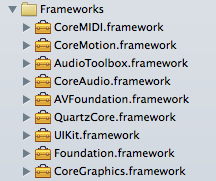
\includegraphics{images/frameworks}
\end{center}
\caption{Required Frameworks for Csound for iOS}\label{fig:frameworks}
\end{figure}

%======

\section{Introduction to the API}
\subsection{CsoundObj and Csound API's}

Csound for iOS is released with the standard Csound C API as well as a custom Objective-C CsoundObj API that has been designed to make developing on iOS convenient.  The CsoundObj API includes methods for binding widgets to channels (used to communicate to and from Csound), mapping hardware MIDI to widgets, enabling hardware sensors, and more.  For further detail, please consult the CsoundObj.h and CsoundObj.m files.

While the CsoundObj API has been designed to ease things for iOS development and to follow conventions of Objective-C, the decision was made to not wrap everything in the Csound C API.  As C coding is commonly found to be used within iOS development, we felt it was better to try to cover the important things that are normally done in Objective-C in CsoundObj, while delegating the user to the C API for parts of Csound that may not be used as often.  The CSOUND* struct pointer that a CsoundObj class holds can be accessed via the \textbf{getCsound} method in CsoundObj.  For more information about the Csound C API, consult the csound.h header file within csound-iOS/headers.

\section{Using the CsoundObj API}

The CsoundObj API revolves around the Objective-C CsoundObj class. This class contains a CSOUND* struct pointer and has methods for running Csound, as well as convenience methods to help aid developers in connecting elements to Csound. By itself, CsoundObj can take in a CSD file and render it.  By using CsoundValueCacheables, objects can interact to read values from and write values to Csound.  Beyond that, extended features can be accessed by using the Csound C API together with the CSOUND* struct.

\subsection{Designing Csound CSD projects to work with Hosts}

To communicate to and from a host program with Csound, you will most likely use \textbf{chnset} and \textbf{chnget} opcodes. These opcodes will allow you to read from and write values to a named channel.  Your host program will also be writing to and reading from these same channels.  As a byproduct of using named channels, your CSD will be portable to work on other platforms (Desktop, Android); porting over apps to/from iOS then will only involve redoing the application and UI code, while your audio engine (Csound) should ``just work.'' 

 

\subsection{CsoundValueCacheable for Communicating with Csound}

The CsoundObj API has been created to ease communication with Csound by using objects that implement the CsoundValueCacheable protocol.  The protocol definition is as follows:

\begin{lstlisting}[caption=CsoundValueCacheable Protocol Definition]
@protocol CsoundValueCacheable

-(void)setup:(CsoundObj*)csoundObj;
-(void)updateValuesToCsound;
-(void)updateValuesFromCsound;
-(void)cleanup;

@end
\end{lstlisting}

CsoundValueCacheables are used to both read values from Csound as well as write values to Csound.  The lifecycle of CsoundValueCacheables is as follows:

\begin{itemize}
\item \textbf{setup} - this method is called after Csound's compile call but before the main performance loop. CsoundValueCacheables should use this method to cache any channel pointers and any other values they will need during performance.
\item \textbf{updateValuesToCsound} and \textbf{updateValuesFromCsound} - these methods are called during the Csound performance loop. \textbf{updateValuesToCsound} is called before each call to csoundPerformKsmps, while \textbf{updateValuesFromCsound} is called after each call. 
\item \textbf{cleanup} - this method is called after Csound has completed its run and should be used by CsoundValueCacheables to free up any allocated data and remove references to channel pointers.
\end{itemize}

By using CsoundValueCacheables, CsoundObj functionality can be extended to communicate with as many items as you would like. The Csound for iOS API contains pre-made wrapper classes for common UI classes (UISlider, UIButton, UISwitch) as well as hardware sensors (Accelerometer, Attitude, Gyroscope).  CsoundObj has helper methods for the CsoundValueCacheables that come with the CsoundObj API, as well as the generic \textbf{addCsoundValueCacheable} and \textbf{removeCsoundValueCacheable} methods for adding custom CsoundValueCacheables. Please consult these classes as well as their use in context within the Csound for iOS Examples project.


%======

\section{Common CsoundObj API Methods}

\subsection{Binding Widgets to CsoundObj}

The CsoundObj API contains the following methods for binding widgets:

\begin{lstlisting}[caption=Methods for Widget Binding]
-(id<CsoundValueCacheable>)addSwitch:(UISwitch*)uiSwitch forChannelName:(NSString*)channelName;
-(id<CsoundValueCacheable>)addSlider:(UISlider*)uiSlider forChannelName:(NSString*)channelName;
-(id<CsoundValueCacheable>)addButton:(UIButton*)uiButton forChannelName:(NSString*)channelName; 
\end{lstlisting}

These methods allow for easy binding of UISwitches, UISliders, and UIButtons, and return the CsoundValueCacheable that was created to wrap the widget. If the design of your app requires that you remove a widget from being used with CsoundObj, you can use the returned CsoundValueCacheable and pass it to the removeCsoundValueCacheable method. To bind your own custom widgets, you will need to create your own CsoundValueCacheable.  There are examples of both using the convenience widget binding methods as well as custom CsoundValueCacheables in the Csound for iOS Examples project.

%======

\section{Interfacing with Hardware}
\subsection{Audio Input and Output}

CsoundObj has been designed to connect everything necessary for audio input and output from Csound to CoreAudio.  Enabling input and output depends on what commandline arguments are given when running Csound.  The commandline arguments should be supplied as part of the CSD's \textbf{CsOptions} section.  To enable audio output, use \textbf{-o dac} and to enable audio input, use \textbf{-i adc}. 

\subsection{MIDI Hardware Input}

MIDI input is supported in two ways: directly to Csound, or indirectly via Widgets. 

\subsubsection{Direct MIDI input to Csound}

CsoundObj has a property called \textbf{midiInEnabled}.  By default this value is set to NO; setting it to YES will enable MIDI input from CoreMIDI directly into Csound. This will allow using Csound's MIDI handling and opcodes to respond to note and controller data from hardware MIDI devices connected to your device (currently limited to iPad devices).  The Csound for iOS Examples project contains an example called \emph{MIDI Test} which demonstrates a project that is setup to handle MIDI coming from a hardware keyboard.

Note, this flag is read when CsoundObj begins a Csound run.  Setting this to YES while CsoundObj is currently rendering will have no effect. 

\subsubsection{Using MidiWidgetsManager to Control Widgets}

For MIDI controller data, rather than handle it directly in Csound, you can use the MidiWidgetsManager to map data from channels to UI Widgets.  The MidiWidgetsManager uses \textbf{MidiWidgetWrappers} to handle mapping of controller data and setting values on widgets.  Currently, the MidiWidgetsManager only has one built-in MidiWidgetWrapper for UISlider. To map values to custom widgets, you will need to create your own implementations of MidiWidgetWrappers. 

This alternative to direct MIDI input to Csound allows for MIDI mapping without a CsoundObj instance actively rendering. In terms of architecture, MIDI values will map to Widgets, and the values within the Widgets are what will be connected with Csound.  By using this design, the values in the widget will be the primary source of values across the system and no synchronization of values is required, whether modified by MIDI or touch input. 

\subsection{Accelerometer, Gyroscope, Attitude}

CsoundObj has built-in support for three of the more commonly used hardware sensors on iOS devices: Accelerometer, Gyroscope, and Attitude. CsoundObj has the following methods to enable these features:


\begin{lstlisting}[caption=CsoundObj Hardware Sensor Methods]
-(id<CsoundValueCacheable>)enableAccelerometer;
-(id<CsoundValueCacheable>)enableGyroscope;
-(id<CsoundValueCacheable>)enableAttitude; 
\end{lstlisting}

When these features are enabled, CsoundValueCacheables that wrap the sensors will send values into Csound via hardcoded channels:

\begin{itemize}

\item Acclerometer
\begin{itemize}
\item accelerometerX
\item accelerometerY
\item accelerometerZ
\end{itemize}

\item Gyroscope 
\begin{itemize}
\item gyroX
\item gyroY
\item gyroZ
\end{itemize}

\item Attitude 
\begin{itemize}
\item attitudeRoll
\item attitudePitch
\item attitudeYaw
\end{itemize}

\end{itemize} 

Once a sensor has been enabled, you can access those values in Csound using \textbf{chnget}. For further study, please see the \emph{Hardware Test} example in the Examples project. 

%======

\section{Csound for iOS Examples}

The Examples project contains a number of simple examples that illustrate different aspects of working with Csound for iOS.  The following is a brief description of each of the examples.

\subsection{Simple Test 1}

Simple example that plays ascending notes.  The pitch of the notes can be altered by using the slider.  Also, a UISwitch is used to turn on/off the rendering of Csound.  In the code, you'll find that the callback that is connected to the UISwitch shows the basic usage of CsoundObj to render a CSD that is included as a resource for the project:

\begin{lstlisting}[caption=Example code showing configuring and starting a CsoundObj]
-(IBAction) toggleOnOff:(id)component {
    UISwitch* uiswitch = (UISwitch*)component;
    NSLog(@"Status: %d", [uiswitch isOn]);
    
    if(uiswitch.on) {
      
        NSString *tempFile = [[NSBundle mainBundle] pathForResource:@"test" ofType:@"csd"];  
        NSLog(@"FILE PATH: %@", tempFile);
        
        [self.csound stopCsound];
        
        self.csound = [[CsoundObj alloc] init];
    [self.csound addCompletionListener:self];
        [self.csound addSlider:mSlider forChannelName:@"slider"];
        [self.csound startCsound:tempFile];
        
    } else {
        [self.csound stopCsound];
    }
}
\end{lstlisting}

\subsection{Simple Test 2}

This is a generative music example that contains a number of sliders that affect the rate of notes generated, the duration of notes, and the ADSR envelope for each note. 


\subsection{Button Test}

This example uses a CSD based on the one used for Simple Test 2, but depends on the user to trigger a button to generate each note.  The two buttons in this example show two different ways in which to integrate buttons with CsoundObj:

\begin{enumerate}
\item Using CsoundObj's \textbf{addButton} method, which will setup a k-rate channel for Csound.  The value will be 0 when the button is not pressed, and will be 1 for one ksmps period when a button is pressed (it returns to 0 the following ksmps period). 
\item Using a standard button callback, the callback will create a string score and send that to Csound using CsoundObj's \textbf{sendScore} method. (See code below.)
\end{enumerate}


\begin{lstlisting}[caption=Example code showing sending score text to CsoundObj]
-(IBAction) eventButtonHit:(id)sender {
    NSString* score = [NSString stringWithFormat:@"i2 0 %f", [mDurationSlider value]];

    [mCsound sendScore:score];
}
\end{lstlisting}

Note that the second method will read the value from the duration slider when creating the note, while the first method handles reading the duration from the channel within the CSD code. 

\subsection{MIDI Test}

This example shows a number of different techniques:

\begin{enumerate}
\item In the \textbf{viewDidLoad}, a \textbf{MidiWidgetsManager} is created and used to map MIDI controller values to sliders.
\item MIDI keyboard and controller input is also routed to Csound using CsoundObj's \textbf{setMidiInEnabled} method. This allows using standard Csound MIDI programming within the context of a Csound for iOS project. (This has been tested on iPad 1 and 2, using a Korg NanoKey connected via Apple USB Camera Connection kit, as well as with MIDI keyboards hooked up to an Alesis I/O Dock.) 
\item A custom multi-touch virtual keyboard widget demonstrates how to track the different touches, map them to keyboard keys, and use \textbf{sendScore} to turn on and off notes. 
\end{enumerate}

For those interested in making virtual instruments, this example may be useful to use as a starting point for your own projects.

\subsection{Ping Pong Delay}

This example shows processing audio input in realtime, using a Ping Pong Delay. The use of audio input is controlled by the standard Csound flag \textbf{-i adc} that is found in the CSD's \textbf{CsOptions} section.  


\subsection{Harmonizer}

This example highlights the same techniques as the Ping Pong Delay, but shows using Csound's streaming Phase Vocoder to create a harmonizer effect. 

\subsection{Hardware Test}

This example shows using hardware sensors.  For this example, the accelerometer is enabled and values are read by the CSD to affect the pitch of a vco2 oscillator, as well as cutoff and resonance of a moogladder filter. 

\subsection{Csound Haiku 4}

\emph{Csound Haiku} is a generative art music work by Iain McCurdy.  Number 4 from this set of pieces was chosen to exercise what is capable on this platform.

\subsection{Record Test}

This example demonstrates the recording feature of CsoundObj.  It also includes a custom metering widget that implements \textbf{CsoundValueCacheable} to read values from Csound.  Note that the \textbf{updateValuesFromCsound} reads the minimum necessary values from Csound and then continues further calculations off the audio callback thread where \textbf{updateValuesFromCsound} is called.  It is important to minimize the amount of processing done in the audio callback thread and to push all processing to another thread.  This can be done using the standard \textbf{performSelector} method; upon completing calculations, updates to the UI will need to be done on the main thread, which is done here using \textbf{performSelectorOnMainThread}.  This pattern is common in audio processing applications. 

\subsection{Multitouch XY}

This example demonstrates a multitouch performance surface. The multi-touch code maps each touch down and up to a note on and off.  It also sends continous x and y values to Csound.  The Csound programming in the CSD shows a technique for doing individual per-note control data mapping by dynamically assigning what channels of data each note should read from. 

\subsection{Waveview}

This example demonstrates using a CsoundValueCacheable to read an f-table from Csound and displaying that table.  Note that the WaveView's code is doing some optimization to check if it has already loaded.  It is also checking that the table itself has completed loading before trying to grab any values for the table. 

\begin{lstlisting}[caption=Waveview code demonstrating reading f-tables from Csound]
- (void)updateValuesFromCsound
{
    if (!tableLoaded) {
        NSAutoreleasePool *pool = [[NSAutoreleasePool alloc] init];

        CSOUND *cs = [csObj getCsound];
        sr = csoundGetSr(cs);
        ksmps = csoundGetKsmps(cs);
        
        if ((tableLength = csoundTableLength(cs, 1)) > 0) {

            table = malloc(tableLength * sizeof(MYFLT));
            csoundGetTable(cs, &table, 1);
            tableLoaded = YES;
            [self performSelectorInBackground:@selector(updataDisplayData) withObject:nil];
        }

        [pool release];
    }

}
\end{lstlisting}

This example also follows the same pattern as the previous example where it off-loads calculations in a background thread using \textbf{performSelectorInBackground}, then posts to the main thread to update the user interface.

\subsection{Audio File Test}

This examples demonstrates a technique of finding the URL of an AIFF file that is packaged as a resource with the project and playing that audio file with Csound.  The example sets up an instance of CsoundObj in its \textbf{viewDidLoad} method, as well as binds a custom UIKnob widget for controlling the playback pitch of the audio file:

\begin{lstlisting}[caption=CsoundObj setup code]
- (void)viewDidLoad
{
    [super viewDidLoad];
    self.csound = [[CsoundObj alloc] init];
    [self.csound addCompletionListener:self];
    NSString *csdPath = [[NSBundle mainBundle] pathForResource:@"audiofiletest" ofType:@"csd"];
    [mPitchKnob setMinimumValue:0.5f];
    [mPitchKnob setMaximumValue:2.0f];
    [mPitchKnob setValue:1.0f];
    [self.csound addValueCacheable:mPitchKnob];
    [self.csound startCsound:csdPath];
}
\end{lstlisting}

The UIKnob widget is custom UIView that is also a CsoundValueCacheable.  It uses a hardcoded Csound channel called "pitch".  After the CsoundObj object is setup and started, performance of the audio file is done in the callback to the Play button press:

\begin{lstlisting}[caption=Play button callback code]
- (IBAction)play:(UIButton *)sender
{
    NSString *audioFilePath = [[NSBundle mainBundle] pathForResource:@"audiofiletest" ofType:@"aif"];
    NSString *score = [NSString stringWithFormat:@"i1 0 1 \"%@\"", audioFilePath];
    [self.csound sendScore:score];
}
\end{lstlisting}

This code finds the path for the \emph{audiofiletest.aif} file that is included with the project, and uses that value to construct a score statement to send to Csound. 

\subsection{Console Output}

This example shows how to use an Objective-C selector as a message callback for Csound through the CsoundObj.  In the example's \textbf{run} method, the call to CsoundObj's \textbf{setMessageCallback} with both the selector to call and the target object is used to route Csound's messages to the example's UITextView:

\begin{lstlisting}[caption=Example of setting message callback]
    [self.csound setMessageCallback:@selector(messageCallback:) withListener:self];
\end{lstlisting}

The message callback selector handles formatting the Csound message using typical C code one will find when using message callbacks with Csound:

\begin{lstlisting}[caption=Message Callback Selector Code]
- (void)messageCallback:(NSValue *)infoObj
{
    NSAutoreleasePool *pool = [[NSAutoreleasePool alloc] init];
    Message info;
    [infoObj getValue:&info];
    char message[1024];
    vsnprintf(message, 1024, info.format, info.valist);
    NSString *messageStr = [NSString stringWithFormat:@"%s", message];
    [self performSelectorOnMainThread:@selector(updateUIWithNewMessage:)
                           withObject:messageStr
                        waitUntilDone:NO];
    [pool drain];
}
\end{lstlisting}

Note: after the message is formatted and converted into an Objective-C NSString from a C char*, a \textbf{performSelectorOnMainThread} is used to update the UI with the message text.  The callback from Csound will not be on the main thread. This step is therefore required as all modifications to the user interface must be done on the main thread. 

\subsection{Pitch Shifter}

This example uses the PVS opcodes to perform pitch shifting on a signal coming in from the microphone on the device.  It uses a custom UIControlXY widget that allows controlling the mix of the wet and dry signal along the x-axis and the amount of pitch shifting along the y-axis.  

%======

\section{Conclusion}

We hope that this document has helped you to become familiar with the design and usage of the Csound for iOS API. The example Objective-C and Csound CSD code should hopefully give you a good starting point for your own musical projects, and we encourage you to take these examples and run with it.  We look forward to hearing your questions and feedback on this API, and most of all, look forward to seeing what you will create with all of this.  Best of luck and enjoy! 

\end{document}
